\documentclass[12pt]{standalone}
\usepackage{tikz}
\usetikzlibrary{shapes.geometric, arrows}
\usepackage{amsmath}

\tikzstyle{node} = [rectangle, text centered, align=center]
\tikzstyle{stealthnode} = [rectangle, text centered, align=center, color=gray]
\tikzstyle{arrow} = [thick,>=stealth]
\tikzstyle{stealtharrow} = [thick,>=stealth, color=gray, dashed]

\tikzstyle{back1} = [xshift=0.8cm, yshift=1.2cm]
\tikzstyle{back2} = [xshift=1.6cm, yshift=2.4cm]
\tikzstyle{back3} = [xshift=2.4cm, yshift=3.6cm]
\tikzstyle{front1} = [xshift=-1.2cm, yshift=-1.8cm]

\newcommand{\drawLinewithBG}[3]
{
    \draw [white,line width=7pt, opacity=1.0]  (#1) -- (#2);
    \draw [#3] (#1) -- (#2);
}

\begin{document}

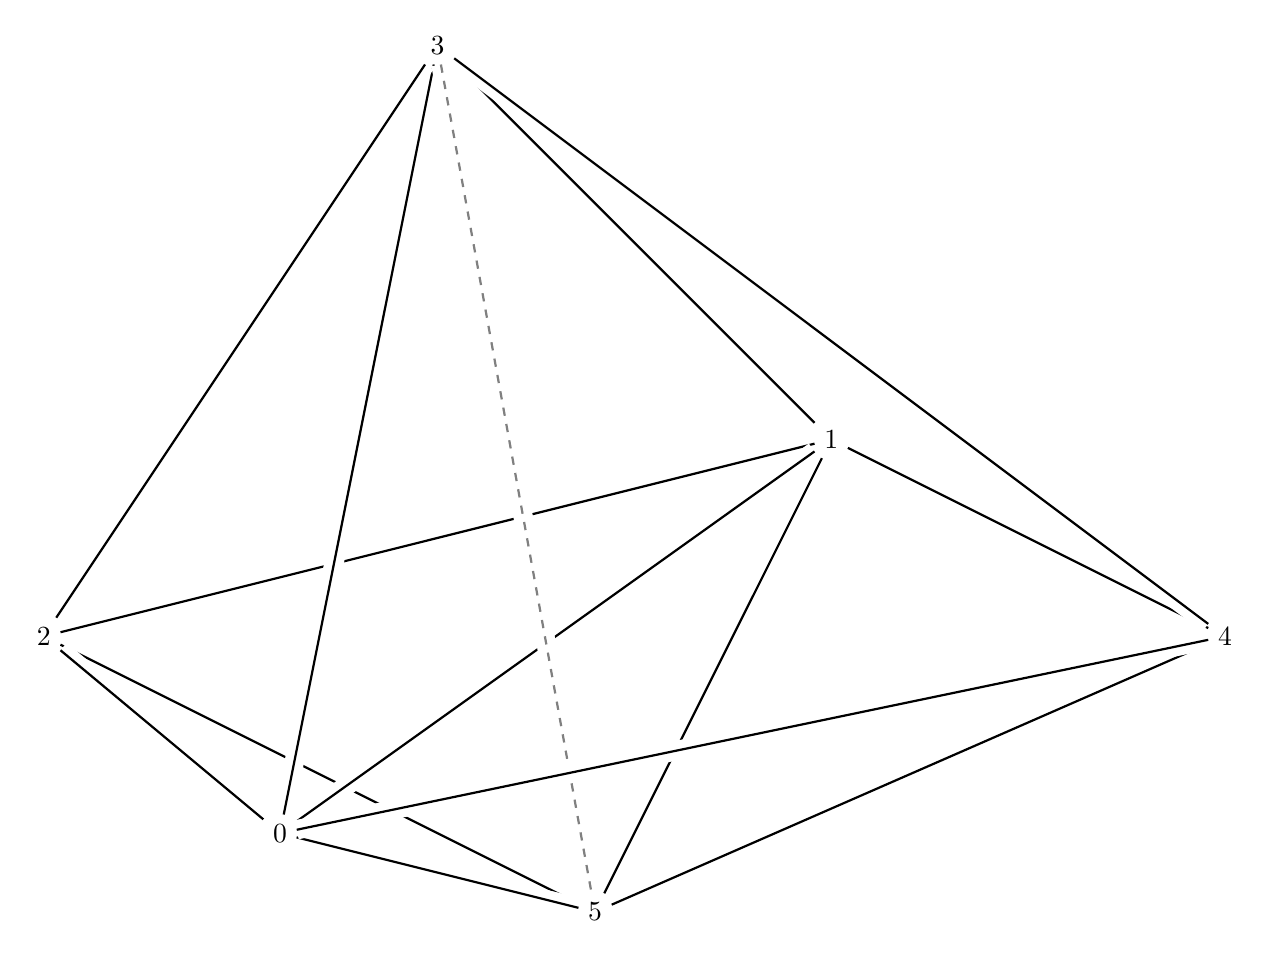
\begin{tikzpicture}[node distance=4.5cm]
\node (v3) [node] {3};
\node (v1) [node, xshift = 5.0cm, yshift=-5.0cm] {1};
\node (v2) [node, xshift = -5.0cm, yshift=-7.5cm] {2};
\node (v0) [node, xshift = -2.0cm, yshift=-10.0cm] {0};
\node (v4) [node, xshift = 10.0cm, yshift=-7.5cm] {4};
\node (v5) [node, xshift = 2.0cm, yshift=-11.0cm] {5};

\drawLinewithBG{v1}{v3}{arrow}
\drawLinewithBG{v1}{v2}{arrow}
\drawLinewithBG{v2}{v5}{arrow}
\drawLinewithBG{v0}{v1}{arrow}
\drawLinewithBG{v0}{v2}{arrow}
\drawLinewithBG{v0}{v3}{arrow}
\drawLinewithBG{v2}{v3}{arrow}

\drawLinewithBG{v1}{v5}{arrow}
\drawLinewithBG{v1}{v4}{arrow}
\drawLinewithBG{v3}{v4}{arrow}

\drawLinewithBG{v0}{v5}{arrow}
\drawLinewithBG{v1}{v5}{arrow}

\drawLinewithBG{v0}{v5}{arrow}
\drawLinewithBG{v4}{v5}{arrow}

\drawLinewithBG{v3}{v5}{stealtharrow}

\drawLinewithBG{v0}{v4}{arrow}

\end{tikzpicture}

\end{document}
